\chapter*{Введение}\label{sec:secIntro}
\addcontentsline{toc}{chapter}{Введение}

\todo
\textbf{Ввести понятие кхд, оно тут несколько раз используется. Описать кварк-глюонную плазму и состояние деконфайнмента. Разобраться с упоминанием NA61 в тексте и таблицах.}

%\textbf{Фазовая диаграмма (что такое и почему нужно ее изучать), физическая программа СBM, и сравнение с другими экспериментами в этой области (по доступной области фазовой диаграммы и наблюдаемым, жесткость требований для детекторов --- в разделе актуальность), подводка к теме работы. Этот раздел не более 5-6 страниц.}

Исследование уравнения состояния ядерного вещества --- одна из важнейших проблем современной физики. В обычных условиях ядерная материя существует в виде нейтронов и протонов, связанных друг с другом благодаря сильному взаимодействию. При изменении плотности и температуры изменяется состояние ядерного вещества, возможны фазовые переходы. Перед учеными стоит задача определить границы существования различных фаз и описать их свойства. Совокупность теоретических представлений по данному вопросу отображается на фазовой диаграмме, см.~\figref{fig:PhaseDiagram}. Здесь по горизонтальной оси отложен барионный химический потенциал $\mu_{B}$, связанный с плотностью барионов $\rho_{B}$, а по вертикальной --- температура $T$. Область высокой температуры и малой плотности соответствует ранней вселенной, когда нуклоны еще не были сформированы. Область больших плотностей и малых температур реализуется в глубине нейтронных звезд. В земных условиях получение сгустка ядерного вещества с повышенными температурой и плотностью, т.н. файербола (fireball), возможно в столкновениях тяжелых ионов. Актуальные экспериментальные исследования направлены на установление границы между барионной материей и кварк-глюонной плазмой (КГП), локализацию критической точки и исследование свойств материи в указанных областях фазовой диаграммы~\cite{CBMBook}. Области фазовой диаграммы в координатах ($T$, $\rho_{B}$) для материи с нулевой странностью и отношением зарядового числа к барионному $Q/B=0.4$, в которых происходит адронизация (hadronic freeze-out) в экспериментах с тяжелыми ионами, показаны на \figref{fig:PhaseDiagram2}. \cite{} \todo источник картинки

\begin{figure}[H]
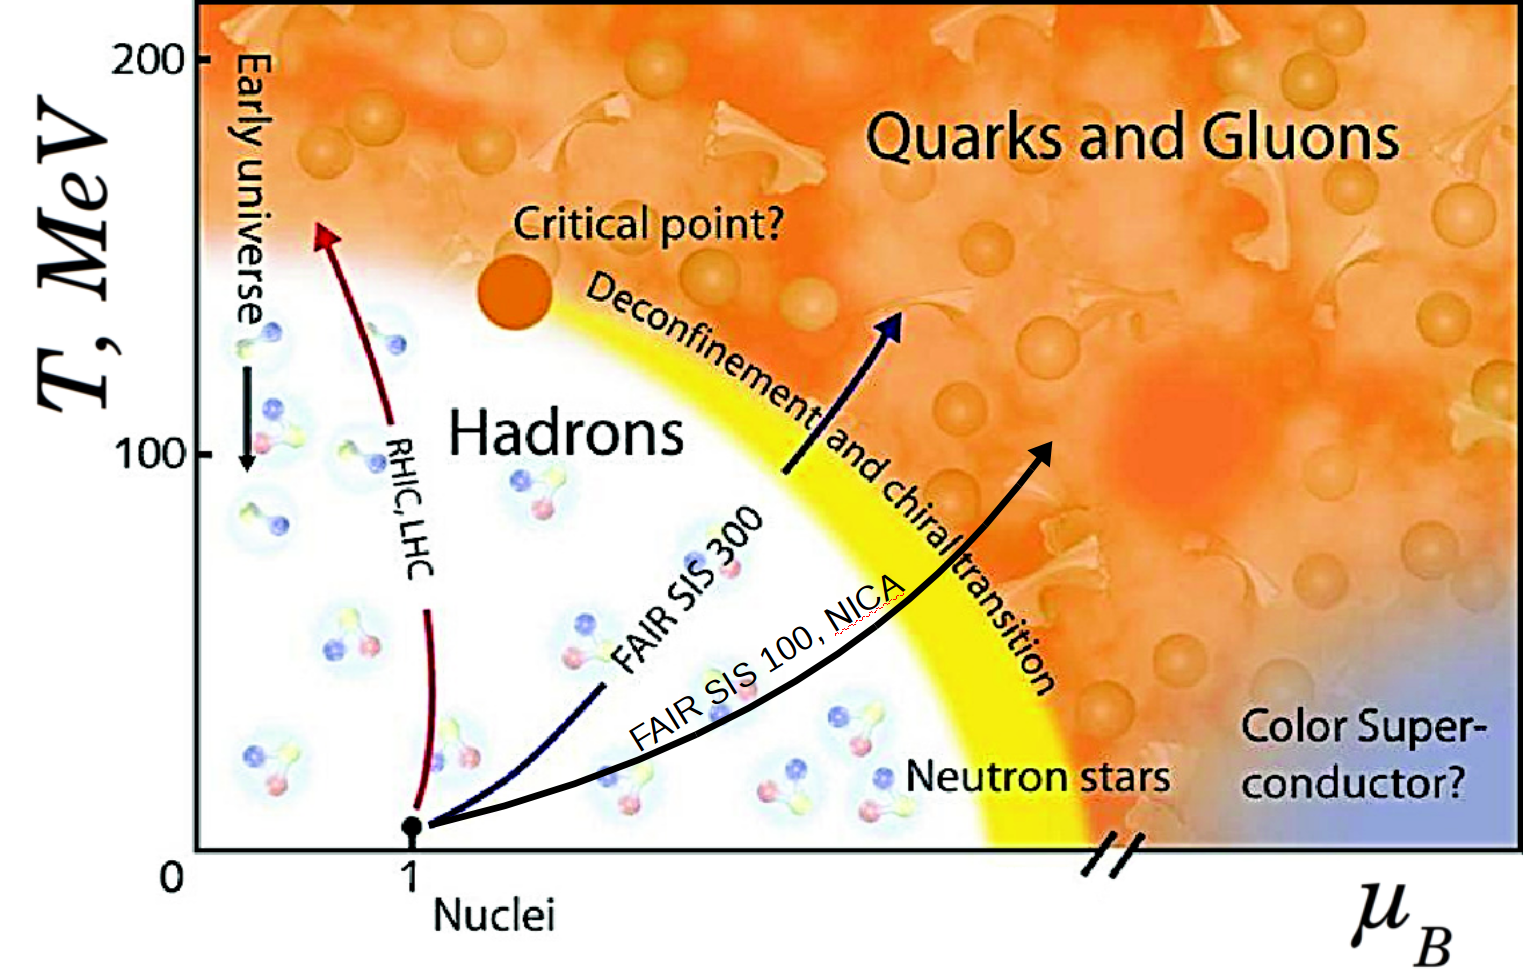
\includegraphics[width=0.8\textwidth]{pictures/qcdPhaseDiagram2.png}
\caption{Фазовая диаграмма барионной материи.}
\label{fig:PhaseDiagram}
\end{figure}

\begin{figure}[H]
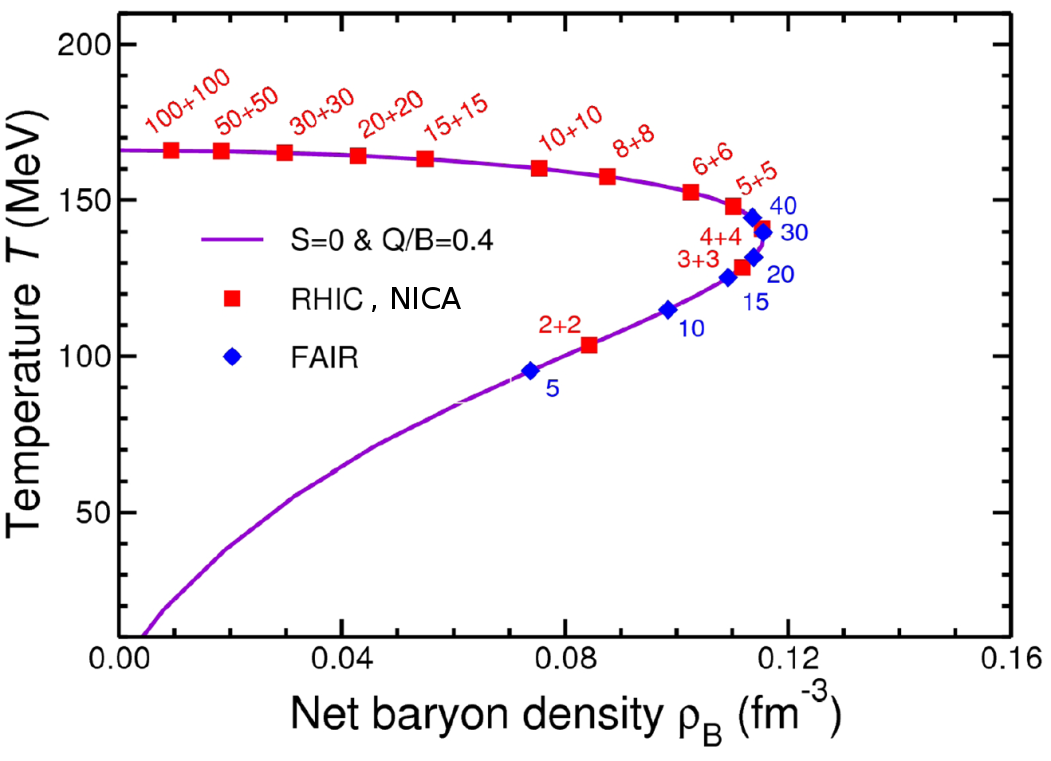
\includegraphics[width=0.8\textwidth]{pictures/Phase_diag.png}
\caption{Фазовая диаграмма барионной материи, по материалам работы~\cite{}. Синий --- режим с фиксированной мишенью на FAIR, красный --- режим встречных пучков на RHIC и NICA}
\label{fig:PhaseDiagram2}
\end{figure}

На~\figref{fig:LittleBang} показана схема эволюции файербола, образованного при столкновении двух тяжёлых ионов в лаборатории.
Информация о свойствах ядерной материи в той или иной области фазовой диаграммы может быть извлечена из анализа наблюдаемых, чувствительных к состояниям, в которых находился файербол в момент ``вымораживания'' тех или иных частиц.

\begin{figure}[H]
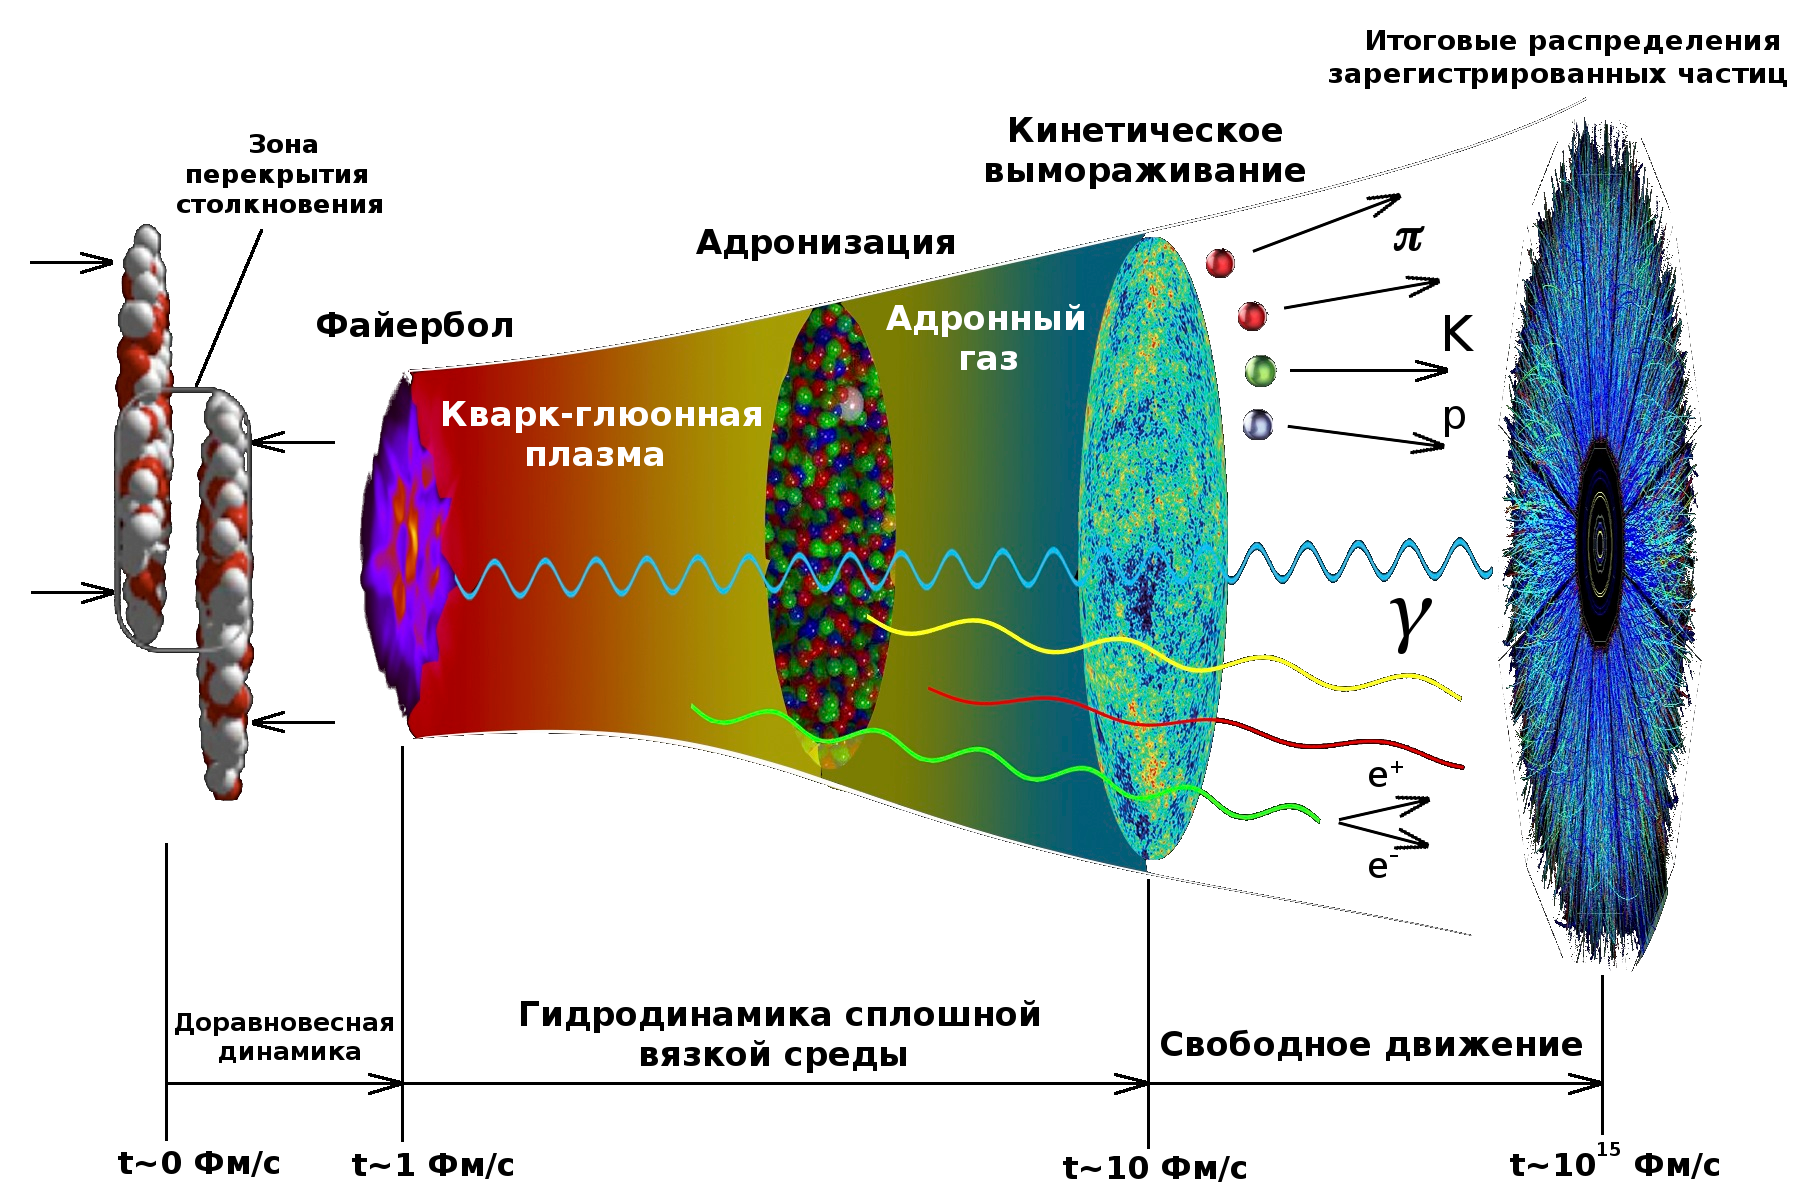
\includegraphics[width=1.0\textwidth]{pictures/little_bang_rus2.png}
\caption{Этапы релятивистского столкновения тяжёлых ионов.}
\label{fig:LittleBang}
\end{figure}

Разные наблюдаемые рождаются на разных этапах столкновения, следовательно, все они несут информацию о разных состояниях вещества, существовавших в разное время после столкновения первичных ионов.

%Особое внимание в CBM уделяется легким векторным мезонам, регистрируемым не напрямую, а по продуктам распада по дилептонным каналам ($e^{+} + e^{-}$ в основном c помощью RICH и $\mu^{+} + \mu^{-}$ в основном c помощью MUCH). Также, можно, например, отметить т.н. прямые фотоны, рождаемые в первые моменты столкновения и регистрируемые электромагнитным калориметром ECAL.

\begin{figure}[H]
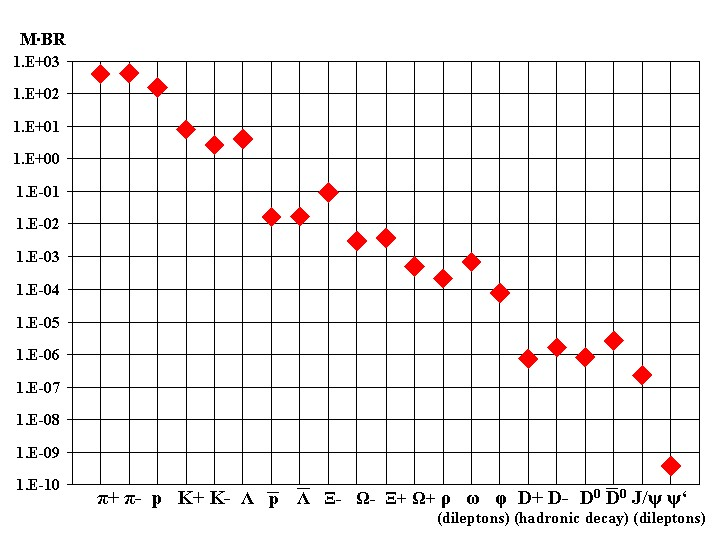
\includegraphics[width=0.8\textwidth]{pictures/CBM_observables.png}
\caption{Основные наблюдаемые CBM. По горизонтальной оси --- восстанавливаемая частица, по вертикальной --- произведение множественности на коэффициент ветвления, характеризующее ожидаемую статистику.}
\label{fig:CBMParticlesYields}
\end{figure}

\todo \textbf{Дать ссылку на источник? Я взял это из CBM Physics Book стр. 866.}


% ------------------------------------------------------------------
% ------------------------------------------------------------------
% ------------------------------------------------------------------


\textbf{СЮДА НАДО СВОДНЫЙ НО НЕ ОЧЕНЬ ПОДРОБНЫЙ СПИСОК НАБЛЮДАЕМЫХ}

\textbf{----------------------------------------------------------------------------------------------------------}

Наблюдаемые MPD. \\
1 этап: \\
Выходы частиц и спектры \\
Флуктуации от события к событию \\
Фемтоскопия, включая $\pi$, $K$, $p$, $\Lambda$ \\
Коллективные потоки и идентификация адронов \\
Электромагнитные измерения ($e$, $\gamma$) \\

2 этап: \\
Полная множественность частиц \\
Изучение асимметрии (лучшее определение плоскости реакции) \\
Точное изучение дилептонов (расширение ECAL) \\
Экзотические частицы (мягкие фотоны, гипер-ядра) \\


Физическая программа CBM нацелена на исследование свойств сверхплотной барионной материи, образующейся в ядро-ядерных столкновениях при энергии пучка от~2~до~45~\GeVperNucl. CBM проектируется с учётом необходимости справляться с измерением высокой статистики адронных, лептонных и фотонных проб в большом аксептансе. Физическая программа включает в себя множество наблюдаемых, среди которых:

\begin{itemize}
\item выход и коллективный поток странных и очарованных адронов; \todo \textbf{ожидается что они отразят процесс становления деконфайнмента};
\item коллективный поток адронов, который особенно чувствителен к уравнению состояния ядерного вещества на ранних стадиях реакций;
\item производство частиц при пороговых энергиях (странность на SIS100 и очарование на SIS300), которое может нести важную информацию об уравнении состояний ядерной материи;
\item нестатистические отклонения от события к событию различных параметров (выходы частиц, отношения выходов), связанные с сохранением квантовых чисел (барионных, заряда, странности), которые могут служить сигналом о критической точке КХД;
\item изменение адронных масс в среде, в частности изменение, предоставляющее ценную информацию о внутренних процессах при ожидаемом восстановлении киральной симметрии в плотной барионной материи.
\end{itemize}

1) The equation-of-state of baryonic matter at neutron star densities.
The relevant measurements are:

Выход адронов в зависимости от энергии.
%The of the collective flow of hadrons which is driven by the pressure created in the early fireball (SIS100);

Выход гиперонов со странностью больше 1.

2) Свойства адронов в среде
Исследование массовых спектров лёгких векторных мезонов в среде.
Выходы и поперечный импульс (не масса) 




\textbf{CBM RICH TDR, секция 1.3}

Физическая программа CBM фокусируется на следующих пунктах:

1) Уравнение состояния барионной материи при плотностях нейтронных звёзд. \\
Соответствующие измерения: \\
1.1) Коллективный поток адронов, который обусловлен давлением в файерболе на раннем этапе (SIS100); \\
1.2) Выход частиц со странностью больше 1 в столкновениях $Au+Au$ и $C+C$ в диапазоне энергий 2--11~\GeVperNucl{} (SIS100).
% At sub-threshold energies, $\Xi$ and $\Omega$ hyperons are produced in sequential collisions involving kaons and $\Lambda$’s, and, therefore, are sensitive to the density in the fireball.

2) Свойства адронов в среде: \\
Восстановление киральной симметрии в плотной барионной среде модифицирует свойства адронов. \\
Соответствующие измерения: \\
2.1) Распределение масс векторных мезонов в среде, распадающихся в лептонные пары в столкновениях тяжёлых ионов в диапазоне энергий 2--45~\GeVperNucl{}. \\
%and for different collision systems
Лептоны являются проникающими \todo probes, несущими информацию из плотного файербола (SIS100, SIS300).
2.2) Распределения выходов и поперечных импульсов очарованных мезонов в столкновениях тяжёлых ионов как функция энергии столкновения (SIS100, SIS300).

3) Фазовый переход между адронной и партонной материями при высоких барионных плотностях. \\
Уже при энергиях SIS100 в центральных столкновениях тяжёлых ионов плотность в фаерболе превышает $\rho_{0}$ в~7~раз. Разрывность или неожиданные отклонения функции возбуждения являются чувствительными наблюдаемыми фазового перехода. \\
Соответствующие измерения: \\
3.1) Функция возбуждения выходов, спектры и коллективный поток частиц с ненулевой странностью в столкновениях тяжёлых ионов в диапазоне энергий 6--45~\GeVperNucl{} (SIS100, SIS300); \\
3.2) Функция возбуждения выходов, спектры и коллективный поток очарованных частиц в столкновениях тяжёлых ионов в диапазоне энергий 6--45~\GeVperNucl{} (SIS100, SIS300); \\
3.3) Функция возбуждения выходов и спектры лпетонных пар в столкновениях тяжёлых ионов в диапазоне энергий 6--45~\GeVperNucl{} (SIS100, SIS300);

\todo Event-by-event fluctuations of conserved quantities like baryons, strangeness, net-charge etc.

3.4) Отклонения от события к событию таких постоянных параметров, как барионы, странность, \todo
в столкновениях тяжёлых ионов как функция от энергии в диапазоне 6--45~\GeVperNucl{} (SIS100, SIS300);

4) Гиперядра, странные ди-барионы и массивные странные объекты. \\
Теоретические модели предсказывают, что в столкновениях тяжёлых ионов при энергиях SIS100 ожидается производство одиночных \todo и двойных \todo гиперядер, странных ди-барионов и тяжёлых мульти-странных короткоживущих объектов путём

5) Механизмы производства очарования, charm propagation и свойства очарованных частиц в плотной ядерной среде. \\
Соответствующие измерения: \\
5.1) Попереченое сечение и спектр импульсов частиц с открытым очарованием ($D$-мезоны) в протон-ядерных столкновениях при энергиях SIS100 и SIS300. Свойства $D$-мезонов в среде могут быть получены из соотношения $T_{A} = (\sigma_{pA} \rightarrow DX) / (A \times \sigma{pN} \rightarrow DX)$, измеренного для различных ядер мишени; \\
5.2) Попереченое сечение, спектр импульсов и коллективный поток частиц с открытым очарованием ($D$-мезоны) в ядерно-ядерных столкновениях при энергиях SIS300; \\
5.3) Попереченое сечение, спектр импульсов и коллективный поток чармония ($J/\psi$) в протон-ядерных и ядерно-ядерных столкновениях при энергиях SIS100 и SIS300.


\textbf{----------------------------------------------------------------------------------------------------------}



% http://www.fair-center.eu/for-users/experiments/nuclear-matter-physics/cbm/introduction.html



% ------------------------------------------------------------------
% ------------------------------------------------------------------
% ------------------------------------------------------------------



Наиболее важные действующие эксперименты в этой области исследований --- это STAR на ускорителе релятивистских тяжелых ионов (RHIC) в Брукхейвене, США, и ALICE на большом адронном коллайдере (LHC) в ЦЕРН, Женева, Швейцария. Отметим также эксперимент предыдущего поколения NA61 (North Area 61 a.k.a. SHINE --- SPS Heavy Ion and Neutrino Experiment) на синхротроне SPS в ЦЕРН. Из строящихся экспериментов наиболее важны MPD на ионном коллайдере NICA в Дубне и CBM на ускорительном комплексе FAIR в Дармштадте, Германия.

HADES (High Acceptance DiElectron Spectrometer) --- эксперимент на SIS18 в GSI, который будет расположен выше по пучку перед CBM, когда последний будет построен.
BM$@$N (Baryonic Matter at Nuclotron) --- эксперимент на нуклотроне в ЛФВЭ ОИЯИ.
BES --- Beam Energy Scan
FXT --- FiXed Target

\todo Дать причину, почему нужно говорить о частоте взаимодействий

\begin{figure}[H]
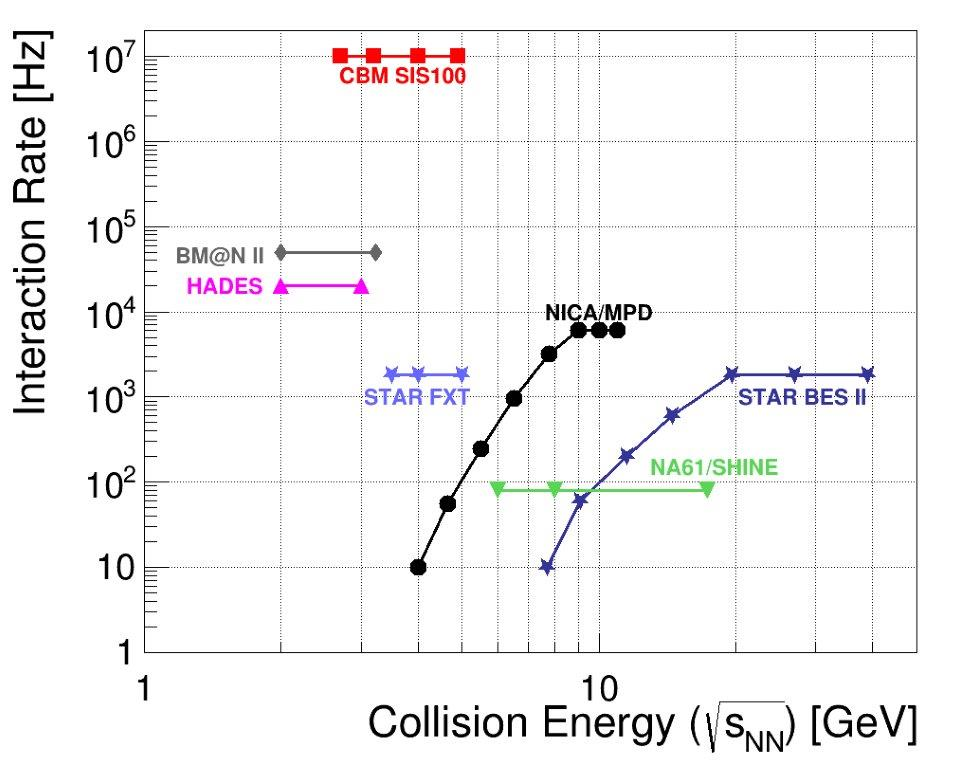
\includegraphics[width=0.8\textwidth]{pictures/Experiments.png}
\caption{Энергии и частоты взаимодействий основных экспериментов физики тяжёлых ионов.}
\label{fig:Experiments}
\end{figure}

% ------------------------------------------------------------------
% ------------------------------------------------------------------
% ------------------------------------------------------------------

%ЗДЕСЬ о том, какую область фазовой диаграммы и какими наблюдаемыми зондирует каждый эксперимент.
%Какая часть фазовой диаграммы и какие наблюдаемые, STAR, ALICE, MPD.
%Теперь еще что надо:
%для Стар и Алиса в наиболее жестком режиме найти
%ионы до (самый тяжелый)
%энергии до
%частота взаимодействия до
%число вторичных частиц на событие до
%если получится (можете написать кому-то и спросить) максимальная угловая плотность частиц.

\section{STAR@RHIC}

% https://www.bnl.gov/npp/docs/tribble090712/Vigdor_RHIC_overview_rev2.pdf - слайд 7

Релятивистский коллайдер тяжёлых ионов (The Relativistic Heavy Ion Collider, RHIC) расположен в Брукхейвенской национальной лаборатории (Brookhaven National Laboratory, BNL), штат Нью-Йорк, США. Первоначально RHIC проектировался для достижения максимально высоких энергий столкновения и предоставлял $\sqrt{s_{NN}}=200$~\GeVperNucl. С целью исследования более широкой области фазовой диаграммы, начиная с 2010~г. выполняется скан вниз по энергиям пучка, называемый Beam Energy Scan (BES).

Детекторная установка STAR (Solenoidal Tracker at RHIC) --- это одна из двух ныне действующих установок на RHIC. Основная задача STAR --- исследование формирования и характеристик кварк-глюонной плазмы.

%\todo \textbf{Здесь описать то, как соотносится FAIR с другими ускорителями, на которых выполняются или планируются эксперименты аналогичные CBM. Здесь появляется фазовая диаграмма, LHC, RHIC, NICA. При этом о самих экспериментах, аналогичных CBM, разговор идёт чуть дальше после описания физической программы CBM. Может быть оставить как есть в следующей секции и ничего тут уж не писать?}

% 1209546.pdf Abstract

В 2011 была завершена первая фаза программы скана с пучками $Au+Au$ с энергий от 7.7~\GeVperNucl{} до 39~\GeVperNucl. Учитывая набранные ранее данные диапазон энергий $\sqrt{s_{NN}}$, измеренных на RHIC составляет 7.7--200~\GeVperNucl. Этот диапазон энергий столкновения соответствует области фазовой диаграммы, в которой ожидается наличие перехода фазового первого рода и критической точки.

%В 2010 и 2011 была выполнена первая фаза программы скана с пучками $Au+Au$ энергий 7.7, 11.5, 19, 27 и 39~\GeVperNucl. Учитывая набранные ранее данные (62, 130 и 200~\GeVperNucl), диапазон энергий $\sqrt{s_{NN}}$, измеренных на RHIC составляет 7.7--200~\GeVperNucl. Этот диапазон энергий столкновения соответствует интервалу $\mu_{B}$ от~20 до~450~МэВ, в котором ожидается наличие перехода фазового первого рода и критической точки.

Вторая фаза BES запланирована на 2018--2019~гг. и будет сфокусирована на пучках $Au+Au$ при энергиях $\sqrt{s_{NN}}$ от~20 до~7~\GeVperNucl{} в режиме встречных пучков и $\sqrt{s_{NN}}$ от~7 до~3.5~\GeVperNucl{} в режиме с фиксированной мишенью (FXT).

% http://iopscience.iop.org/article/10.1088/1742-6596/455/1/012037/pdf

%In 2010 and 2011 RHIC completed phase I of the Beam Energy Scan (BES) program with data sets at 7.7, 11.5, 19, 27 and 39 GeV. This is complemented by the data collected earlier at higher energies (62, 130 and 200 GeV). Together they cover the $\mu_{B}$ interval from 20 to 450 MeV, which is believed to contain the range associated with the first order phase transition and CP.

%В исходной статье есть картинка.

% https://arxiv.org/pdf/1211.1350.pdf   section 2

%\textbf{Редактировать!}

Эти измерения, несмотря на низкую статистику, позволят измерить выходы и спектры адронов и определить, опираясь на статистическую термальную модель (THERMUS~\cite{}) параметры состояния на границе химического вымораживания, называемого также адронизация.

%Ключевые характеристики ($T$, $\mu_{B}$) исследуемой области фазовой диаграммы могут быть извлечены из результатов измерений выходов адронов в столкновениях тяжёлых ионов. В первой фазе BES поперечный импульс определяется для $\pi$, $K$, $p$, $\Lambda$, $\Xi$, $K^{0}_{S}$ и $\phi$. Отношения выходов частиц используются для нахождения условий ``химического вымораживания'' (адронизация) (состояния, когда устанавливаются выходы частиц) с помощью статистической термальной модели (THERMUS).

%\textbf{Редактировать!}

% Два ключевых параметра --- температура $T_{ch}$ и барионный потенциал $\mu_{B}$ ``химического вымораживания''.

%These quantities can be extracted from the measured hadron yields. Transverse momentum spectra for the BES Phase-I energies are obtained for $\pi, K, p, \Lambda, \Xi, K^{0}_{S}$, and $\phi$. The particle ratios are used to obtain the chemical freeze-out (a state when the yields of particles get fixed) conditions using the statistical thermal model (THERMUS). The two main extracted parameters are chemical freeze-out temperature $T_{ch}$ and $\mu_{B}$. 

% https://www.epj-conferences.org/articles/epjconf/pdf/2015/14/epjconf_icnfp2014_01009.pdf
% Страница 2 - есть таблица с энергиями и количеством событий

% sonia_kabana_talk_excitedQCD_final.pdf
% Слайд 31

% \begin{table}[H]
% \caption{}
% \label{tabl:RHICenergies}
% \begin{tabular}{ | p{0.3\linewidth} | p{0.3\linewidth} | p{0.3\linewidth} | }
% \hline
% Энергия (\GeVperNucl) & Кол-во событий (млн.) & Время (недели) \\
% \hline
% 200 & 350 & 11 \\
% \hline
% 62.4 & 67 & 1.5 \\
% \hline
% 39 & 130 & 2 \\
% \hline
% 27 & 70 & 1 \\
% \hline
% 19.6 & 36 & 1.5 \\
% \hline
% 14.5 & 20 & 3 \\
% \hline
% 11.5 & 12 & 2 \\
% \hline
% 7.7 & 4 & 4 \\
% \hline
% \end{tabular}
% \end{table}

% ------------------------------------------------------------------
% ------------------------------------------------------------------
% ------------------------------------------------------------------

%\section{ALICE@LHC}

Эксперимент ALICE (A Large Ion Collider Experiment), один из четырёх крупных экспериментов на большом адронном коллайдере (Large Hadron Collider, LHC) ЦЕРН, нацелен на изучение столкновений тяжёлых ионов. Рекордная энергия $\sqrt{s_{NN}}=5.5$~\mbox{ТэВ/нуклон} для сталкивающихся пучков ядер свинца позволяет получить ядерную материю с беспрецедентно высокой температурой. Частота взаимодействий достигает порядка 10~кГц. В эксперименте одновременно сохраняются данные с тремя типами триггеров: с минимальным перекрытием ядер, с высокой центральностью и с отбором редких событий заданного типа.

Высокая температура ядерного вещества приводит к следующим особенностям: процессы с высокой передачей энергии идут с высокой вероятностью, что позволяет тестировать модели пертурбативной КХД; появляется возможность регистрировать $Z^{0}$ и $W^{\pm}$ бозоны, рождающиеся в окружении горячей ядерной материи; возрастает относительное время существования КГП, в результате чего расширение фаербола определяется в большой степени динамикой партонов, что проявляется в потоках и спектрах испускаемых адронов; большое значение приобретает регистрация прямых фотонов, несущих информацию о термодинамических условиях на ранней горячей фазе столкновения. Среди интересных результатов, полученных к настоящему моменту на ALICE, отметим компенсацию подавления рождения $J/\psi$ в столкновениях с высокой центральностью. Этот эффект может быть связан с большой концентрацией очарованных кварков и антикварков в среде в момент адронизации. Температура адронизации, достигнутая в ALICE оценивается как T$\approx$160~MeV.

% http://www.slac.stanford.edu/econf/C060717/papers/L010.PDF

%Эксперимент ALICE (A Large Ion Collider Experiment) --- это один из четырёх крупных экспериментов на большом адронном коллайдере (Large Hadron Collider, LHC), который занимается изучением столкновений тяжёлых ионов.

%The rate of Pb--Pb collisions in 2010 and 2011 was well below the ALICE limits and ALICE was able to take data at the highest achievable luminosity, on the order of $10^25$ $s^{-1}$ $cm^{-2}$ in 2010 and $10^{26}$ $s^{-1}$ $cm^{-2}$ in 2011, with the corresponding hadronic $\mu$ being on the order of $10^{-5}$ -- $10^{-4}$ and $10^{-4}$ -- $10^{-3}$, respectively.

%During the 2011 Pb--Pb running period, the interaction rate provided by the LHC reached 3-4 kHz. ALICE ran with the minimum bias, centrality, and rare triggers activated at the same time. In the LHC Run 2 (2015--2017), for which the expected collision rate is O(10) kHz, still low enough to avoid pileup.

%The LHC at CERN will provide colliding Pb ions with an energy of $\sqrt{s_{NN}}=5.5 TeV$.

%It is expected that the LHC can deliver luminosities of $10^{27}$ $cm^{2}$ $s^{-1}$ for Pb--Pb collisions, which results in a minimum-bias interaction rate of 8~kHz. Lighter ions can be delivered with higher luminosities of up to $10^{29}$ $cm^{2}$ $s^{-1}$, corresponding to an interaction rate of several 100~kHz. The machine can deliver p--p luminosities up to $10^{31}$ $cm^{2}$ $s^{-1}$ but because of detector limitations this luminosity is restricted to $10^{30}$ $cm^{2}$ $s^{-1}$ for ALICE.

%--- Hard processes become abundant.
%The abundance of hard processes at the LHC will allow for precision test of perturbative QCD. In addition, the large jet rates at the LHC permit detailed measurements of jet quenching to study the early stages of the collision.

%--- Access to weakly interacting hard probes.
%Direct photons as well as $Z^{0}$ and $W^{\pm}$ bosons produced in hard processes will provide information about nuclear parton distributions at high $Q^{2}$ . Jet tagging with such probes yields a calibrated energy scale for jet quenching studies.

%--- Fireball expansion is dominated by parton dynamics.
%Due to the expected longer lifetime of the QGP, the parton dynamics will dominate over the hadronic contribution to the fireball expansion and the collective features of the event.

%The charged particle multiplicity per colliding nucleon pair measured by ALICE for the most central collisions is double that measured at RHIC, where the collision energy is factor 14 lower, fig.1. This shows that the system created at LHC has much higher energy density and is at least 30\% hotter that at RHIC. Fig. 2 shows the charged particle multiplicity as a function of the number of participants. 

%One of the classic signals expected for a quark-gluon plasma (QGP) is the radiation of ``thermal photons'', with a spectrum reflecting the temperature of the system. With a mean-free path much larger than nuclear scales, these photons leave the reaction zone created in a nucleus–nucleus collision unscathed. So, unlike hadrons, they provide a direct means to examine the early hot phase of the collision. However, thermal photons are produced throughout the entire evolution of the reaction and also after the transition of the QGP to a hot gas of hadrons. In the PbPb collisions at the LHC, thermal photons are expected to be a significant source of photons at low energies (transverse momenta, $p_{T}$, less than around 5~\GeVoverC{}). The experimental challenge in detecting them comes from the huge background of photons from hadron decays, predominantly from the two-photon decays of neutral pions and ? mesons. 

%Direct photons are defined as photons not coming from decays of hadrons, so photons from initial hard parton-scatterings (prompt photons and photons produced in the fragmentation of jets) --- i.e. processes already present in proton-proton collisions --- contribute to the signal. Indeed, for pT greater than around 4~\GeVoverC{}, the measured spectrum agrees with that for photons from initial hard scattering obtained in a next-to-leading-order perturbative QCD calculation. For lower pT, however, the spectrum has an exponential shape and lies significantly above the expectation for hard scattering, as the figure shows. The inverse slope parameter measured by ALICE, $T_{LHC}$ = 304$\pm$51 (stat.+syst.) MeV, is larger than the value observed in gold-gold collisions at $\sqrt{s}$ = 0.2~TeV at Brookhaven’s Relativistic Heavy-Ion Collider (RHIC), $T_{RHIC}$ = 221 $\pm 19$ (stat.) $\pm 19$ (syst.) MeV. In typical hydrodynamic models, this parameter corresponds to an effective temperature averaged over the time evolution of the reaction. The measured values suggest initial temperatures well above the critical temperature of 150--160 MeV (approx. 1.8 $\times$ 1012 K) at which the transition between ordinary hadronic matter and the QGP occurs. The ALICE measurement also indicates that the LHC has produced the hottest piece of matter ever formed in a laboratory. 

%At the LHC, however, extremely interesting developments are expected. In particular, a much higher number of charm-anticharm pairs are produced in the nuclear interaction, thanks to the unprecedented centre-of-mass energies. As a consequence, even a suppression of the $J/\psi$ yield in the hot QGP phase could be more than counter-balanced by a statistical combination of charm-anticharm pairs happening when the system, after expansion and cooling, finally crosses the temperature boundary between the QGP and a hot gas of particles. If the density of heavy quark pairs is large enough, this regeneration process may even lead to an enhancement of the $J/\psi$ yield --- or at least to a much weaker suppression with respect to the experiments at lower energies. The observation of the fate of the $J/\psi$ in nuclear collisions at the LHC constitutes one of the goals of the ALICE experiment and was among its main priorities during the first run of the LHC with lead beams in November/December 2010.

%The results from the first ALICE run are rather striking, when compared with the observations from lower energies. While a similar suppression is observed at LHC energies for peripheral collisions, when moving towards more head-on collisions --- as quantified by the increasing number of nucleons in the lead nuclei participating in the interaction --- the suppression no longer increases. Therefore, despite the higher temperatures attained in the nuclear collisions at the LHC, more $J/\psi$ mesons are detected by the ALICE experiment in Pb--Pb with respect to p--p. Such an effect is likely to be related to a regeneration process occurring at the temperature boundary between the QGP and a hot gas of hadrons (T$\approx$160~MeV).


% ------------------------------------------------------------------
% ------------------------------------------------------------------
% ------------------------------------------------------------------

\section{------------------------}

Эксперименты на RHIC и LHC исходно были нацелены на изучение ядерной материи при высоких температурах и относительно малых значениях барионного потенциала. Большой физический интерес представляет и область фазовой диаграммы с высокой барионной плотностью, которая может быть исследована при столкновениях тяжелых ядер с меньшей энергией. Пионерские исследования в этой области делаются на ускорителе RHIC в программе сканирования по энергиям (\todo ввести BES тут). Недостатком этих исследований является невысокая частота взаимодействий, что позволяет получить доступ к только ограниченному кругу наблюдаемых. Существуют два пути повышения частоты взаимодействий: (1) оптимизация ускорителя встречных пучков под низкие энергии, что позволит минимизировать эмиттанс пучка при большом значении тока и, следовательно, увеличить частоту взаимодействий и (2) работа с фиксированной мишенью. Первый подход реализуется в проекте MPD на ускорителе NICA в Дубне, а второй --- в проекте CBM на FAIR в Дармштадте.

% ------------------------------------------------------------------
% ------------------------------------------------------------------
% ------------------------------------------------------------------

\section{MPD@NICA}

Эксперимент MPD на строящемся ускорителе NICA в ОИЯИ предназначен для исследования столкновений тяжелых ионов с энергией в диапазоне $\sqrt{s_{NN}}$ от~4 до~11~\GeVperNucl{} со светимостью порядка $10^{27}$~см$^{-2}$~с$^{-1}$. Помимо выходов и спектров адронов, эксперимент позволит измерить флуктуации от события к событию, исследовать анизотропию выходов адронов и осуществить корреляционные измерения при высокой статистике.

% Sorin_SQM2013_Birmingham_25_07_2013.pdf

В Объединённом Институте Ядерных Исследований (ОИЯИ) в г.~Дубне идёт строительство коллайдерного комплекса на базе нуклотрона NICA (Nuclotron-based Ion Collider fAciliy), который предоставит пучки от протонов до ионов золота в диапазоне энергий $\sqrt{s_{NN}}$ от 4 до 11~\GeVperNucl. При этом светимость для $^{197}Au$ составит $1.5 \cdot 10^{26}$ см$^{-2}$ с$^{-1}$ для $\sqrt{s_{NN}}=4$~\GeVperNucl{} и $10^{27}$ см$^{-2}$ с$^{-1}$ для $\sqrt{s_{NN}}=11$~\GeVperNucl.


% слайд 23

$pi^{+}$, $K^{+}$, $p$, $\rho$, $\omega$, $\phi$, $\Omega$, $D^{0}$, $J/\psi$



% ------------------------------------------------------------------
% ------------------------------------------------------------------
% ------------------------------------------------------------------

\section{CBM@FAIR}

Эксперимент с фиксированной мишенью CBM нацелен на исследование ядерной материи с высокой барионной плотностью с рекордной статистикой. Частота ядерных взаимодействий в этом эксперименте будет достигать $10^7$~с$^{-1}$ при $\sqrt{s_{NN}}$ \todo. В центральных столкновениях плотность может превышать нормальную ядерную в 8--10 раз. Благодаря высокой статистике с точностью, недоступной в других экспериментах, в CBM \todo такие наблюдаемые как: флуктуации потоков и спектров адронов от события к событию; анизотропия потоков адронов, в т.ч. странных и очарованных; выходы вблизи порога и свойства в среде лёгких векторных мезонов, $J/\psi$, $D$-мезонов. Все наблюдаемые могут быть измерены при различных значениях энергии столкновения и центральности, которая характеризует величину фаербола.

В экспериментах в ЦЕРНе и Брукхейвенской национальной лаборатории поиск критической точки осуществляется только посредством регистрации спектральных характеристик потоков вторичных частиц нескольких типов, рождающихся в большом количестве. Эксперименты FAIR, благодаря высокой интенсивности первичных пучков, открывают дополнительную возможность регистрировать редкие события со сканированием обширной области фазовой диаграммы по энергиям частиц. В частности планируется впервые непосредственно исследовать признаки возникновения ``огненного шара'' (fireball) --- области ядерной материи, в которой произошёл переход от барионной фазы к кварк-глюонной фазе, --- с помощью регистрации короткоживущих векторных мезонов, распадающихся на дилептонные пары.

Диапазон энергий FAIR 2--35~\GeVperNucl{} для ионов золота хорошо подходит для проведения экспериментов в области фазовой диаграммы с высокими плотностями ядерной материи, превосходящими нормальную плотность в 8--10 раз.

\todo \textbf{В разных источниках числа расходятся. Где-то 35, где-то 45...}

Высокая интенсивность пучка и продолжительная его доступность позволят CBM впервые измерять редкие пробы, такие как очарованные адроны и лёгкие векторные мезоны (с помощью дилептонных распадов), в области энергий, предоставляемых FAIR.

Экспериментальная задача CBM --- измерять перечисленные наблюдаемые в A+A, p+A, p+p столкновениях как функцию энергии столкновения и размера системы с высокой точностью и статистикой, а также искать нарушения непрерывностей, которые могут служить сигналом о фазовом переходе первого уровня. Данная физическая программа будет выполняться измерением ядерных столкновений при экстремально высоких частотах взаимодействия.

% ------------------------------------------------------------------

\section{------------------------}

В таблицу~\ref{tabl:Experiments1} сведены такие базовые параметры рассмотренных выше экспериментов, как энергия в центре масс и частота взаимодействий.

\begin{table}[H]
\caption{Показатели экспериментов в области сверхплотной материи}
\label{tabl:Experiments1}
\begin{tabular}{ | p{0.23\linewidth} | p{0.35\linewidth} | p{0.32\linewidth} | }
\hline
Эксперимент & Диапазон энергий (Au/Pb) & Частота взаимодействий, Гц \\
\hline
STAR$@$RHIC BNL & $\sqrt{s_{NN}}$=7--200 \GeVperNucl & 1--800 \\
\hline
NA61$@$SPS CERN & $E_{kin}$=20--160 \GeVperNucl \newline $\sqrt{s_{NN}}$=6.4--17.4 \GeVperNucl & 80 \\
\hline
ALICE$@$LHC CERN & \todo & \todo \\
\hline
MPD$@$NICA JINR & $\sqrt{s_{NN}}$=4--11 \GeVperNucl & 7000 \\
\hline
CBM$@$FAIR GSI & $E_{kin}$=10--35 \GeVperNucl \newline $\sqrt{s_{NN}}$=2.7--8.3 \GeVperNucl & $10^5$--$10^7$ \\
\hline
\end{tabular}
\end{table}

%Sorin_SQM2013_Birmingham_25_07_2013.pdf

\begin{table}[H]
\caption{Наблюдаемые в области высокой плотности барионов}
\label{tabl:Experiments2}
\begin{tabular}{ | p{0.28\linewidth} | p{0.15\linewidth} | p{0.15\linewidth} | p{0.15\linewidth} | p{0.15\linewidth} | }
\hline
\textbf{Наблюдаемые} & \textbf{STAR$@$RHIC} \newline \textbf{BNL} & \textbf{NA61$@$SPS} \newline \textbf{CERN} & \textbf{MPD$@$NICA} \newline \textbf{JINR} & \textbf{CBM$@$FAIR} \newline \textbf{GSI} \\
\hline
Адроны & $+$ & $+$ & $+$ & $+$ \\
\hline
Корреляции, флуктуации \newline при высокой статистике & & & $+$ & $+$ \\
\hline
Дилептоны & & & & $+$ \\
\hline
Очарованные \newline частицы & & & & $+$ \\
\hline
\end{tabular}
\end{table}

%\begin{table}[H]
%\caption{Наблюдаемые в области высокой плотности барионов}
%\label{}
%\begin{tabular}{ | p{0.22\linewidth} | p{0.10\linewidth} | p{0.32\linewidth} | p{0.14\linewidth} | p{0.16\linewidth} | }
%\hline
%\textbf{Эксперимент} & \textbf{Адроны} & \textbf{Корреляции,} \newline \textbf{флуктуации при} \newline \textbf{высокой статистике} & \textbf{Дилептоны} & \textbf{Очарованные} \newline \textbf{частицы} \\
%\hline
%STAR$@$RHIC BNL & $+$ & & & \\
%\hline
%NA61$@$SPS CERN & $+$ & & & \\
%\hline
%MPD$@$NICA JINR & $+$ & $+$ & & \\
%\hline
%CBM$@$FAIR GSI & $+$ & $+$ & $+$ & $+$ \\
%\hline
%\end{tabular}
%\end{table}

Данная работа посвящена методическим разработкам для детектора RICH эксперимента CBM, участвующего в измерении таких наблюдаемых как распады легких векторных мезонов ($\rho$, $\omega$, $\phi$) и $J/\psi$-частицы по диэлектронному каналу.

\section*{Актуальность работы:}

Современные эксперименты в области физики высоких энергий и, особенно, столкновения релятивистских тяжелых ионов выдвигают жёсткие требования к проектным решениям при создании установок по причине высокой загрузки, высокой плотности потока частиц и высокой радиационной нагрузки, сложности и многопараметричности моделей, описывающих изучаемые эффекты, тонкости последних и высоких фонов.

Например, (рассказать c конкретными цифрами про загрузки, наблюдаемые (измеримые величины) и фоны в ряде экспериментов, в частности, flow measurements и rare probes в CBM, что-то обязательно про СТАР, АЛИСУ и какой-нибудь еще эксперимент с фиксированной мишенью, подчеркнуть особенности и жесткость требований CBM).

Все эти факторы

Требуются совершенные методы моделирования детекторов с высоким уровнем детализации и возможностью выполнения нескольких итераций расчетов, а также разработка новых систем сбора данных, адекватных современному аппаратному обеспечению и ожидаемым потокам информации.

Кроме того, необходимы интенсивные исследования прототипов создаваемых детекторов.

В настоящей диссертации обсуждаются все три перечисленных аспекта (развернуть на 1-2 абзаца) в применении, в первую очередь, к детектору Черенковских колец эксперимента CBM (далее CBM RICH).

\section*{Цели:}

\begin{itemize}
\item{разработать инструментарий для облегчения создания детальных геометрических моделей, предназначенных для таких сред Монте-Карло моделирования прохождения частиц через вещество, как Geant4 и ROOT, а также для обмена геометрической информацией между этими средами и САПР CATIA~v5;}
\item{создать гибкое и точное описание детектора CBM RICH в среде CbmRoot и осуществить на основе этого описания оптимизацию конструкции и компоновки данного детектора;}
\item{создать ПО для испытания прототипа системы считывания и сбора данных детектора CBM RICH в составе полнофункционального прототипа указанного детектора на пучковых тестах;}
\item{провести исследование свойств прототипа системы считывания и сбора данных детектора CBM RICH на основе результатов пучковых тестов и измерений на лабораторном стенде.}
\end{itemize}

\section*{Научная новизна и практическая ценность работы:}

\begin{enumerate}
\item Разработана схема отображения иерархии геометрии, используемой в моделировании транспорта частиц методом Монте-Карло (МК), на дерево построений САПР CATIA~v5.
\item В среде CATIA~v5 создан набор шаблонов для примитивов и сущностей конструктивной твердотельной геометрии, принятой в системах МК моделирования детекторов.
\item Создан набор инструментов для полуавтоматического построения детальной МК геометрии на основе САПР модели и быстрого обмена геометрией между САПР CATIA~v5 и пакетами МК моделирования GEANT и ROOT.
\item Выполнены беспрецедентно точные параметризованные описания ряда приборов и детекторов в средах МК моделирования.
\item На основе детального параметризованного описания геометрии CBM~RICH выполнена оптимизация компоновки детектора. 
\item Собран прототип системы считывания и сбора данных детектора CBM~RICH.
\item Разработано программное обеспечение для приема, упаковки и передачи бестриггерного потока данных с прототипа системы считывания и сбора данных с частотой до 20~МГц.
\item Разработано программное обеспечение для калибровки точного времени и относительных задержек каналов в потоке данных с детектора CBM RICH.
\item Разработано программное обеспечение для построения событий из бестриггерного потока данных с детектора CBM~RICH в среде CbmRoot.
\item Проведены пучковые тесты прототипа системы считывания и сбора данных в составе полнофункционального прототипа детектора CBM~RICH и дополнительные тесты на лабораторном стенде. 
\item Проведено комплексное исследование свойств канала считывания и сбора данных для CBM~RICH, реализованного на основе многоанодного ФЭУ H12700 с системой динодов ``metal channel'', специально разработанных передней электроники типа предусилитель-дискриминатор и высокоточного ВЦП с последующим прямым вводом данных в единую среду моделирования, сбора и анализа данных CbmRoot.
\item Исследованы временные свойства нанесенного на окно МА~ФЭУ сместителя спектра при возбуждении черенковскими фотонами.
\item Изучены возможности работы канала считывания при пониженных порогах.
\item Проведен сравнительный анализ особенностей считывания многоанодного ФЭУ временным и аналоговым трактами.
% \item Исследованы характеристики детектора CBM~RICH с учетом неидеальности геометрии и шумов электроники.
\end{enumerate}

\section*{На защиту выносятся следующие результаты:}

\begin{enumerate}
\item Разработка методологии и реализация ``CATIA-GDML geometry builder'', средства построения сложной, основанной на инженерном дизайне геометрии детекторов для моделирования прохождения и взаимодействия частиц.
\item Применение ``CATIA-GDML geometry builder'' для построения беспрецедентно точного параметризованного описания геометрии CBM~RICH в среде CbmRoot.
\item Реализация прототипа системы считывания и сбора данных CBM~RICH и проведение его тестов на пучке в составе полнофункционального прототипа этого детектора а также дополнительных тестов на лабораторном стенде.
\item Разработка алгоритмов и программного обеспечения для приема, упаковки и передачи бестриггерного потока данных, для калибровки точного времени и относительных задержек каналов и для построения событий из потока данных с детектора CBM RICH в среде CbmRoot.
\item Результаты комплексного исследования временных свойств канала считывания и сбора данных для CBM~RICH, реализованного на основе многоанодного ФЭУ H12700 с системой динодов ``metal channel'', специально разработанных передней электроники типа предусилитель-дискриминатор и высокоточного ВЦП с последующим прямым вводом данных в единую среду моделирования, сбора и анализа данных CbmRoot.
\item Исследование временных свойств нанесенного на окно МА ФЭУ сместителя спектра при возбуждении черенковскими фотонами.
\item Сравнительный анализ особенностей считывания многоанодного ФЭУ временным и аналоговым трактами.
% \item Исследование характеристик детектора CBM~RICH с учетом неидеальности геометрии и шумов электроники.
\end{enumerate}

\section*{Представление основных положений и результатов}

% Приведено в обратном хронологическом порядке. Можно перегруппировать по важности.

Основные положения и результаты работы докладывались и обсуждались на научных семинарах ЛИТ ОИЯИ и на различных международных конференциях и совещаниях, в том числе:

\begin{enumerate}

\item Семинар НОВФ ЛИТ ОИЯИ, Дубна, Россия, 22.12.2016 \\
Устный доклад ``Development of the readout and DAQ system for CBM RICH and EXPERT. 'CATIA-GDML geometry buidler' and Monte-Carlo geometry of CBM RICH.''

\item Семинар ``Contribution of the young Russian scientists into the project FAIR'', ИТЭФ, Москва, Россия, 14-15.12.2016 \\
Устный доклад ``Detailed study of the stability and uniformity of the CBM RICH readout and DAQ prototype characteristics. Development and application of the Monte Carlo geometry package''

\item Международная конференция ``The 9th International Workshop on Ring Imaging Cherenkov Detectors (RICH 2016)'', Блед, Словения, 05-09.09.2016 \\
Представлен постер ``Development of the CBM RICH readout electronics and DAQ''

\item Международная конференция ``The 20th IEEE-NPSS Real Time Conference (IEEE-NPSS RT2016)'', Падуя, Италия, 05-10.06.2016 \\
Представлен постер ``Development of the CBM RICH readout and DAQ''

\item Международная конференция ``The XX International Scientific Conference of Young Scientists and Specialists (AYSS-2016)'', ОИЯИ, Дубна, Россия, 14-18.03.2016 \\
Устный доклад ``Development and characterization of CBM RICH readout and DAQ''

\item Семинар ``Contribution of the young Russian scientists into the project FAIR'', ИТЭФ, Москва, Россия, 15-17.12.2015 \\
Устный доклад ``Development of 'CATIA-GDML geometry builder' and CBM RICH software''

\item Международное совещание ``26th CBM Collaboration Meeting'', Прага, Чехия, 14-18.09.2015 \\
Устный доклад ``PADIWA test measurements, beamtime analysis (TOT, WLS time resolution)''

\item Международное совещание ``25th CBM Collaboration Meeting'', ГСИ, Дармштадт, Германия, 20-24.04.2015 \\
Устный доклад ``Beamtime analysis: FLIB readout, TOT, timing''

\item Семинар ``Contribution of the young Russian scientists into the project FAIR'', ИТЭФ, Москва, Россия, 12-13.11.2013 \\
Устный доклад ``Modernization of simulation and data acquisition packages of CBM experiment''

\item Международная конференция ``20th International Conference on Computing in High Energy and Nuclear Physics (CHEP)'', Амстердам, Нидерланды, 14-18.10.2013 \\
Представлен постер ``Development and application of CATIA-GDML geometry builder''

\end{enumerate}

\section*{Публикации}


\section*{Личный вклад:}

\todo
\section*{Структура и содержание}\label{sec:secStructureAndContent}

Диссертация состоит из настоящего введения, пяти глав и заключения.

В первой главе
описываются условия эксплуатации, компоновка и основные свойства детекторов эксперимента CBM;
обсуждается важность точного описания и оптимизации конструкции детекторов в свете жёстких условий эксплуатации;
формулируется задача разработки инструментария для обмена геометрической информацией между САПР и средами Монте-Карло моделирования прохождения частиц через вещество (Geant4/ROOT) и облегчения создания детальных геометрических моделей для Geant4/ROOT;
детально описывается конструкция детектора CBM RICH и проводится сравнение с аналогичными приборами из ряда других экспериментов;
формулируются конкретные задачи, связанные с описанием геометрии детектора CBM RICH в среде Монте-Карло;
обсуждается концепция системы считывания и сбора данных эксперимента CBM и воплощение этой концепции в системе считывания и сбора данных детектора CBM RICH;
формулируется задача на исследование прототипа системы считывания и сбора данных указанного детектора.

Во второй главе
обсуждаются некоторые наиболее распространённые способы представления геометрических моделей в ЭВМ, используемые в различном ПО для решения различных вычислительных задач;
рассматриваются предпосылки и принципы создания инструментария, так называемого ``CATIA-GDML geometry builder'', для обмена геометрической информацией между САПР и средами Монте Карло моделирования прохождения частиц через вещество (Geant4/ROOT) и облегчения создания детальных геометрических моделей для Geant4/ROOT;
обсуждаются реализация отображения примитивов и иерархии объемов Geant4/ROOT на дерево построений в среде CATIA~v5 и набор созданных макропрограмм, входящих в ``CATIA-GDML geometry builder'';
описывается методика применения ``CATIA-GDML geometry builder'' и приводятся некоторые примеры.

Третья глава
посвящена применению пакета ``CATIA-GDML geometry builder'' для детектора CBM RICH. В ней подробно рассмотрены задачи, требующие точного описания геометрии механических конструкций детектора и системы крепления и позиционирования зеркал, учета эффектов, связанных с отклонением позиционирования зеркал от номинального, размещения и экранирования от магнитного поля фотодетекторов. Описаны созданные параметризованные геометрические модели и проведенные с их помощью исследования свойств детектора CBM RICH. Кроме того, даются рекомендации по эффективному применению использованного инструментария.

В четвёртой главе
описаны архитектура бестриггерной системы считывания и сбора данных CBM RICH, разработанные модули ПО, необходимые для сбора и анализа данных, а также экспериментальные установки, позволившие осуществить всестороннее исследование прототипа указанной системы.

Пятая глава
посвящена анализу данных пучковых и лабораторных тестов прототипа детектора CBM RICH и результатам исследования свойств и характеристик прототипа системы считывания и сбора данных. Здесь же, на основании проведенных исследований, даются рекомендации по модификации следующей версии прототипа системы считывания и сбора данных.

В заключении приводятся основные результаты работы и выражаются благодарности.

